\chapter{Theoretical and experimental basics}
\label{theory}

\section{The Standard Model of Particle Physics}

The Standard Model of Particle Physics summarizes the current knowledge of fundamental particles and their interactions. The model holds at scales of 1 fm and below. Gravity, being the fourth fundamental force is not included because it is negligible for most phenomena at this scale.

The current view is that all matter is made out of three kinds of elementary particle being leptons quarks and mediators.
There are six leptons falling into three families according to charge, electron number, muon number and tau number. 

Similiar to that there are six flavors of quarks separated by Strangeness (S), charm (C), Beauty (B), and truth (T). As well as the leptons the quarks fall into three generations.
For both kinds of particles the mass rises with the generations and every generation comes as a doublet. The first particle of each lepton doublet is not charged and referred to as a neutrino while the second particle has charge -1.
For each quark doublet there is an element with fractional charge $-\frac{1}{3}$ and an element with fractional charge $\frac{2}{3}$.
To every of these particles there is an anti particle with opposite charge.

The third kind of particle included in the standard model is the mediator. Mediators are gauge bosons whose exchange allows the particles to interact. There are four kinds of of elemtary interactions of which the strong electromagnetic and weak interaction are included in the model. The fourth interaction is the gravitational interaction.
The gauge particles for the strong interaction are the gluons carrying colour charge, the electromagnetic mediator is the photon ($\gamma$) and the weak mediators are the $W^{\pm}$ and $Z$ bosons 


\begin{table}[]
\centering
\caption{Lepton properties}
\label{lepton properties}
\begin{tabular}{l|l|l|l|l|l|}
\cline{2-6}
                                   & symbol        & Charge $Q$ & $L_e$ & $L_{\mu}$ & $L_{\tau}$ \\ \cline{2-6} 
\multirow{2}{*}{First generation\{}  & $e$             & -1       & 1    & 0          & 0           \\ \cline{2-6} 
                                   & $\nu_e$        & 0        & 1    & 0          & 0           \\ \cline{2-6} 
\multirow{2}{*}{Second generation\{} & $\mu$           & -1       & 0    & 1          & 0           \\ \cline{2-6} 
                                   & $\nu_{\mu}$  & 0        & 0    & 1          & 0           \\ \cline{2-6} 
\multirow{2}{*}{Third generation\{}  & $\tau$          & -1       & 0    & 0          & 1           \\ \cline{2-6} 
                                   & $\nu_{\tau}$ & 0        & 0    & 0          & 1           \\ \cline{2-6} 
\end{tabular}
\end{table}

\begin{table}[]
\centering
\caption{Quark properties}
\label{quark properties}
\begin{tabular}{l|l|l|s|l|l|l|l|l|l|}
\cline{2-10}
                                      & Symbol & Charge Q       & mass       & D  & U & S  & C & B  & T \\ \cline{2-10} 
\multirow{2}{*}{First generation \{}  & $d$    & $-\frac{1}{3}$ & 4.8 MeV    & -1 & 0 & 0  & 0 & 0  & 0 \\ \cline{2-10} 
                                      & $u$    & $\frac{2}{3}$  & 2.3 MeV    & 0  & 1 & 0  & 0 & 0  & 0 \\ \cline{2-10} 
\multirow{2}{*}{Second generation \{} & $s$    & $-\frac{1}{3}$ & 95 MeV     & 0  & 0 & -1 & 0 & 0  & 0 \\ \cline{2-10} 
                                      & $c$    & $\frac{2}{3}$  & 1275 MeV   & 0  & 0 & 0  & 1 & 0  & 0 \\ \cline{2-10} 
\multirow{2}{*}{Third generation \{}  & $b$    & $-\frac{1}{3}$ & 4180 MeV   & 0  & 0 & 0  & 0 & -1 & 0 \\ \cline{2-10} 
                                      & $t$    & $\frac{2}{3}$  & 173210 MeV & 0  & 0 & 0  & 0 & 0  & 1 \\ \cline{2-10} 
\end{tabular}
\end{table}

\begin{table}[]
\centering
\caption{Mediator properties}
\label{mediator properties}
\begin{tabular}{|l|l|l|l|l|}
\hline
Interaction     & Theory & Mediator        & Charge          & Coupling  \\ \hline
Strong          & QCD    & gluons (8)      & colour          & 1         \\ \hline
Electromagnetic & QED    & photon $\gamma$ & electric charge & $10^{-1}$ \\ \hline
Weak            & GSW    & $W^{\pm}, Z$    & weak isospin    & $20^{-6}$ \\ \hline
\end{tabular}
\end{table}

Given this the standard model of particle physics has been a very successful model for a very long time and still holds for most cases.
Nevertheless the model has some commonly known weaknesses and does not claim to be complete. For example the gravitational force is not included and in the standard model neutrinos are massless.

Should there be an outline here ? 





\section{The LHC and ATLAS}

The analysis for this thesis has been performed in the ATLAS collaboration. The ATLAS-Detector is one of the four big experiments at the LHC at Cern. Therefore this chapter gives a brief overview over the LHC and ATLAS focusing on the properties directly relevant for Particle Flow Analysis.

After a description of the ATLAS detector in general I will give a little bit more information about the detector components directly relevant for the explanation of particle flow being the tracking detector and the calorimeter. To make the advantages of particle flow understandable to the reader I will give a general description of these detectors and their properties

\subsection{The LHC}

The Large Hadron Collider ("LHC") at CERN was built to extend the frontiers of modern particle physics by delivering high luminosities and unprecedented high energies.\\
The LHC is designed to collide bunches of up to \num{d11} protons
\begin{figure}[htbp]
  \centering
  \includegraphics[width=\figwidth]{CERN_all-experiments}
  \caption[Sketch of the LHC ring, the position of the experiments and
  the surrounding countryside.]{Sketch of the LHC ring, the position
    of the experiments and the surrounding countryside. The four big
    LHC experiments are indicated. The location of the injection lines
    and the SPS are also shown.}
  \label{fig:LHC}
\end{figure}


\subsection{The ATLAS Detector}

The ATLAS detector is built to take advantage of the high energy available at the LHC to observe highly massive particles that lower energy accelerators were not able to create and that way bring new physics theory beyond the standard model of particle physics.

\begin{figure}[htbp]
  \centering
  \includegraphics[width=\figwidth]{atlas-detector}
  \caption[Sketch of the ATLAS detector]{Sketch of the ATLAS detector \cite{atlasfigures}}
  \label{fig:atlas}
\end{figure}


\subsection{Tracking detectors}

The go to method to measure the momenta of charged particles is the usage of tracking detectors.

These detectors are based on charged particles leaving a track of ionisations in any given medium and therefore by detecting this ionizations being able to reconstruct the particles trajectory.
There are two main categories for tracking detectors in use. The first one uses a large gaseous volume in a strong electric field and filled with a structure of wires. The electric field lets the liberating electrons drift towards the wires where they cause a detectable signal.
However the second kind of detectors is based on semiconductor technology and used in most modern detectors like ATLAS. Therefore I will give this kind of tracking detectors a deeper discussion.
introduce semiconductors
explain what happens
what does the field do



\subsection{Calorimeter}

In particle physics a calorimeter is a device to measure first and foremost measure the total energy of a particle. Most of the time also some position information is taken.
Most particles loose all their momentum crossing the calorimeter-structure. Measuring the energy deposited this way gives a measurement for the particle's energy.
Usually a particle deposits its energy by initiating a particle shower. the showers energy is then collected and measured.
Calorimeters are distinguished by the main interaction of the particles one wants to detect. 
\subsubsection{Electromgnetic Calorimeter}






\section{The Particle Flow Algorithm}

Recently only either the Calorimeter or the tracker information was used to reconstruct Jets in ATLAS events. The Particle Flow Algorithm combines tracker and calorimeter information to achieve better resolution especially at lower energies. The main advantages of including the tracker information into reconstruction are listed here:


\begin{itemize}
\item For low energy charged particles the momentum resolution of the tracking detector is superior to the calorimeter.
\item The Tracking detector is able to reconstruct softe particles, which would not pass the noise threshold of the calorimeter.
\item The ATLAS traking detector has a superior angular resolution for single charged particles.
\item Low $p_T$ charged particles may be swept out of the cone before reaching the calorimeter by the magnetic field. The tracker information allows to cluster these particles into the jet.
\item a better vertex determination could lower the pileup-contribution.
\end{itemize}

The advantages of Particle Flow have already been shown for Run 1 data in

\begin{figure}[htbp]
  \centering
  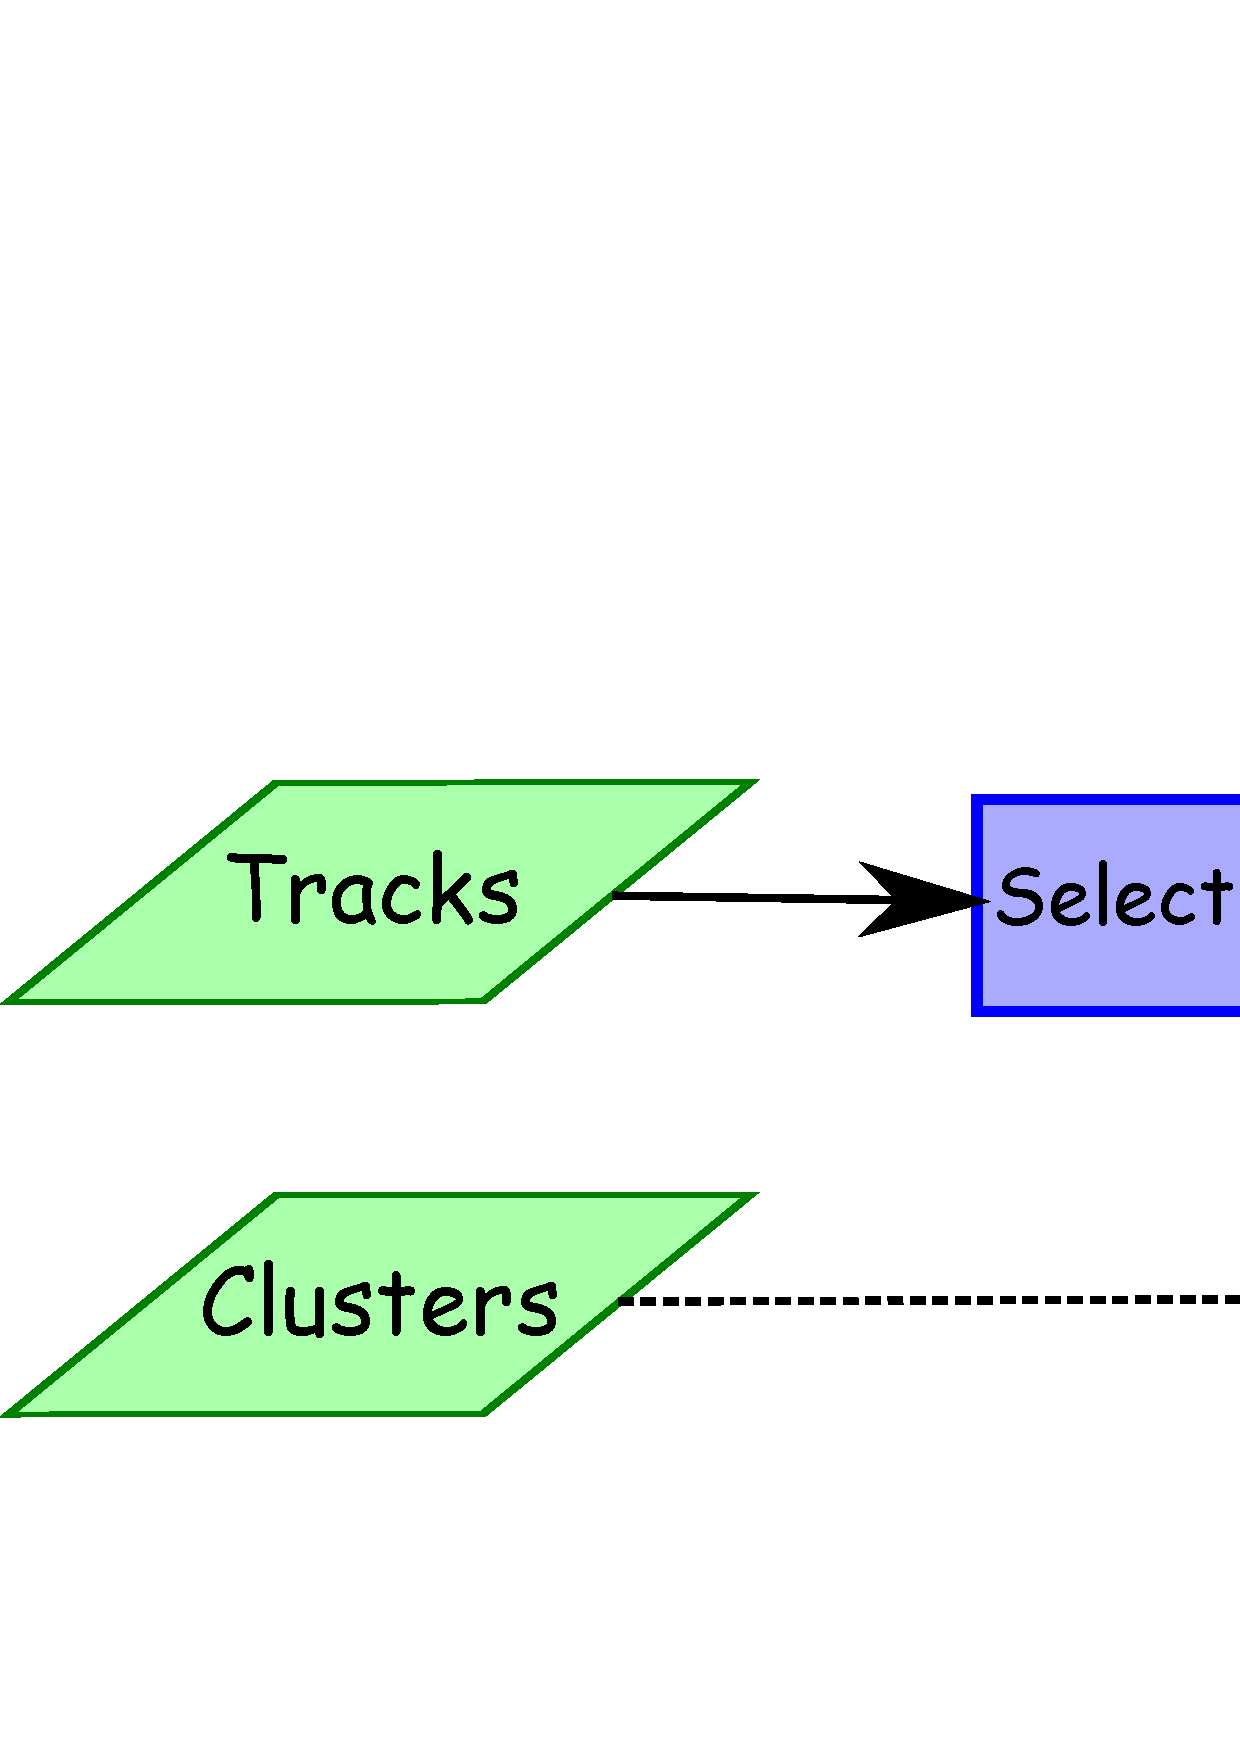
\includegraphics[width=\figwidth]{flowchart.pdf}
  \caption[Flowchart of the steps of the Particle Flow algorithm]{Flowchart of the steps of the Particle Flow algorithm}
  \label{fig:pflowflowchart}
\end{figure}

\subsection{Track selection}



\subsection{Clustering}

The algorithm uses information from the tracker and the calorimeter as input. The information from the calorimeter is give as topological clusters. The construction of these clusters is briefly described in this chapter to give the reader a basic understanding which input information the algorithm uses.
Every cluster is being constructed around a so called seed cell. A seed cell is a cell for which the deposited energy exceeds the expected noise by four times the standard deviation. If a seed is found all the neighboring cells which exceed the noise by at least two times the standard deviation are added to the cluster. Lastly all the cells neighboring these clusters are also added.


\subsection{Matching Track to Cluster}

The algorithm tries to match every track to one or more calorimeter clusters. First the algorithm tries to match a single best-match topo-cluster to every selected track.
To do so first the distances in $\Delta \phi$ and $\Delta \eta$ from the track are extrapolated to the second layer of the EM calorimeter and then topo clsuter. then the topo-clusters get ranked based on the metric:

\begin{equation}
\Delta R' = \sqrt{\left(\frac{\Delta \phi}{\sigma_{\phi}}\right)+\left(\frac{\Delta \eta}{\sigma_{\eta}}\right)}
\end{equation}

where $\sigma_{\eta}$ and $\sigma_{\phi}$ refer to the angular topo-cluster width, computed from the standard deviation of the displacemtens of the topo clusters 

\subsection{Cell Subtraction}

The last step in the Particle Flow algorithm after matching a set of topo-clusters to a track is the cell-wise subtraction of energy deposits to remove remnants and determine which energy deposits belong to the given particle.
If the energy deposited in the set of clusters falls below the expected energy the clusters are simply removed. Otherwise, a cell by cell subtraction is performed.

The first step of the cell subtraction is generating a shower shape from the extrapolated track. Around the extrapolated track rings in $\eta$, $\phi$ space are generated, being just wide enough to independently contain at least one one cell from the extrapolated position. Furthermore the rings are restricted to one layer and for each layer have the same radial size.
After the generation of rings in each layer the average energy density in each ring is computed and the rings are ranked by energy density in descending order. The layer is not used in any way for this ranking.
The subtraction then starts from the ring with highest energy density and proceeds successively to rings in lower order until the next ring's energy exceeds or falls below.
If the ring's energy exceeds the energy still to be substracted the energy in each cell is scaled down by the fraction needed to reach the expected energy then the process halts and the remaining cells are removed as remnants.
An example of the process is sketched in fasofoifjaor


\begin{figure}[htbp]
  \centering
  \begin{subfigure}[b]{0.3\figwidth}
    \includegraphics[width=0.25\figwidth]{a}
    \caption{}\label{fig:sub-a}
  \end{subfigure}
  \begin{subfigure}[b]{0.3\figwidth}
    \includegraphics[width=0.25\figwidth]{b}
    \caption{}\label{fig:sub-b}
  \end{subfigure}
  \begin{subfigure}[b]{0.3\figwidth}
    \includegraphics[width=0.25\figwidth]{c}
    \caption{}\label{fig:sub-c}
  \end{subfigure}
  \begin{subfigure}[b]{0.3\figwidth}
    \includegraphics[width=0.25\figwidth]{d}
    \caption{}\label{fig:sub-d}
  \end{subfigure}
    
    
  \begin{subfigure}[b]{0.3\figwidth}
        \includegraphics[width=0.25\figwidth]{e}
        \caption{}\label{fig:sub-e}
  \end{subfigure}
  \begin{subfigure}[b]{0.3\figwidth}
        \includegraphics[width=0.25\figwidth]{f}
        \caption{}\label{fig:sub-f}
  \end{subfigure}
  \caption{Example of cell subtraction \cite{pflowpaper}}
  \label{fig:sub}
\end{figure}

%add a reference here. wildcard there





\section{Calibration in Particle Flow and its difficulties at the time}

Here I want to explain what tools are used for PFlow already and what tools are missing.
Then I should focus on which tools have been implicitly upgraded
Problematic right now are the cleaning the trigger matching the pileup reweithing and the complete JES